\chapter{Introduction}
\label{ch:introduction}
	Forest covers approximately 30\% of the global land surface, while approximately 50\% of the global forest area is covered by tropical forest \citep{WWF2016}. Tropical forests covering the global land surface between 23$^\circ$ north (the tropic of Cancer) and 23$^\circ$ south (the tropic of Capricorn) around the equator as figure \ref{fig:tropicalzone} shows. This zone comprises several different forest types like tropical rain forest, tropical moist forest, tropical dry forest, and tropical mountain system forest. The distribution and extent of this forest types is affected by the following environmental properties: precipitation levels and seasonality, temperature profile, elevation, and soil characteristics. Rain forest account for approximately 60\% of the tropical forest cover and is characterized by warm and wet climate, while the average annual temperature is above 20 degrees and the precipitation ranges between 2500 and 4500 mm y$^{-1}$. The canopy is dense and dominated by trees with a height between 30 and 45 m. The required climate conditions are typically found between 10$^\circ$ north and 10$^\circ$ south. Tropical forest is a crucial part of our earth system as important factor for climate, water cycle, soil health, biodiversity storage, and source of natural goods for human subsistence. These forests are a major carbon sink and stimulate precipitation. Further, these forests house the largest diversity of species and a large amount of endemic species. However, this unique ecosystem is endangered by forest loss and transitions to other \ac{LULC} types \citep{WWF2016}.
	\begin{figure}[ht]
		\centering
		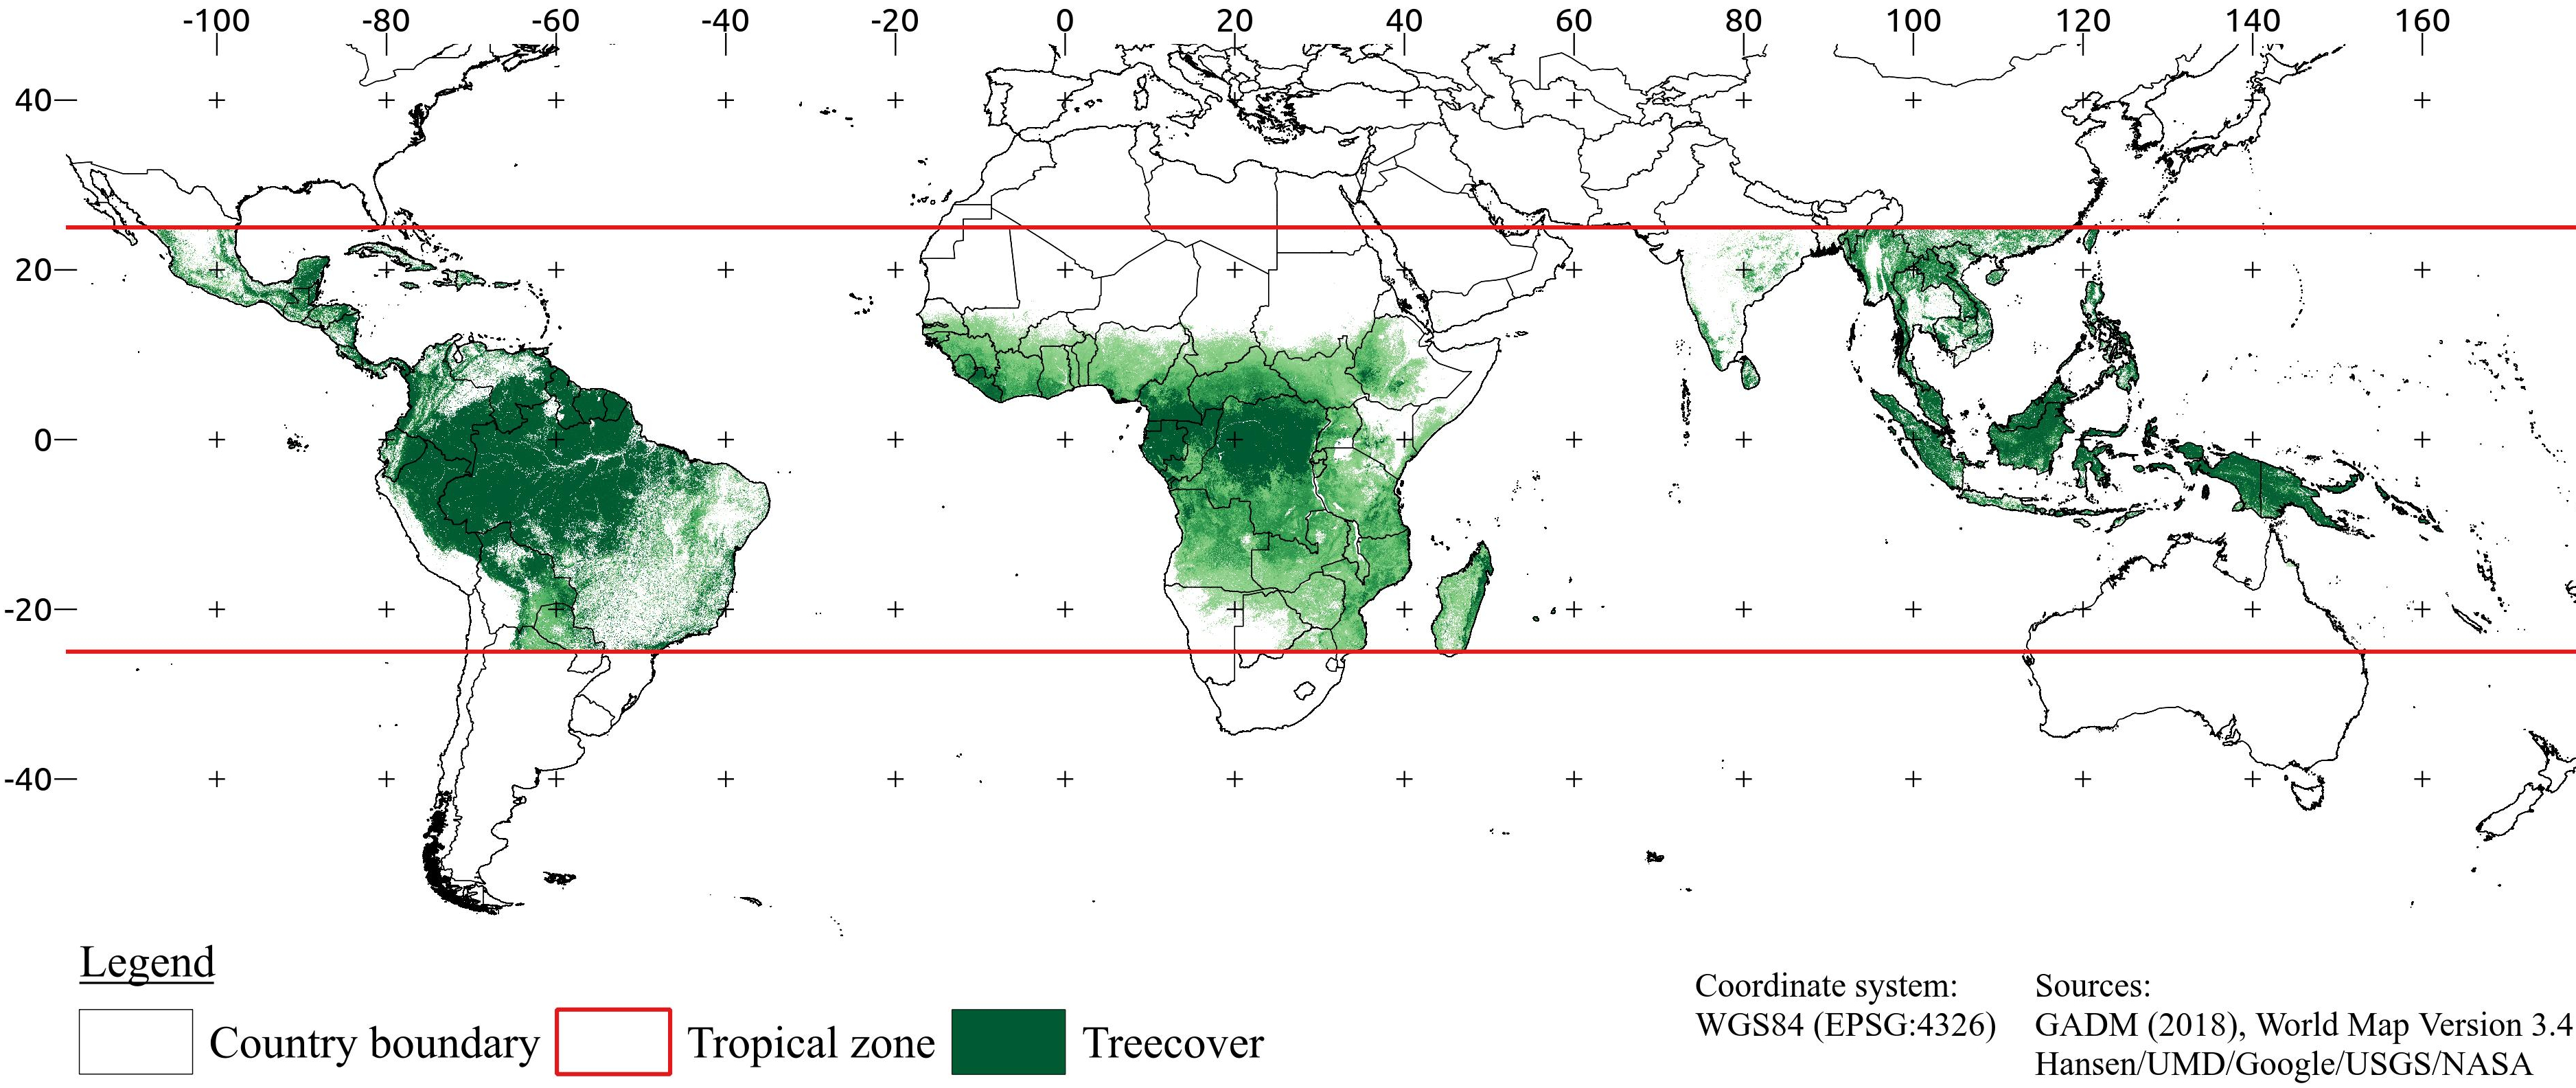
\includegraphics[scale=.97]{img/intro_overview_frameless}
		\caption[Tropical zone and forest]{\textbf{Tropical zone and forest}}
		\label{fig:tropicalzone}
	\end{figure}

	Since the 1990s approximately 3.1\% of the global forest area is lost, while approximately 35\% of the tree cover loss is within tropical forest cover \citep{FAO2016}. Between 1990 and 2015 all the top ten countries with the highest annul net loss of forest are located in the tropical zone \citep{FAO2010,FAO2016}. Forest loss or deforestation is defined as the removal of trees or forest stands from land surface which is subsequently converted to another \ac{LULC}. \citet{Geist2001} introduced the conceptual framework of proximate, underlying, and other causes of tropical deforestation to classify the drivers of forest cover change. Direct deforestation driver or proximate deforestation driver are anthropogenic actions that change forest to other \ac{LC} types. Proximate causes of deforestation are grouped into three different categories: agricultural expansion, wood extraction, and infrastructure expansion. Examples for deforestation driven by agriculture are the expansion of pastures, cropland, and tree crops as shown in figure \ref{fig:deforestationexamples}. Examples for wood extraction and infrastructure expansion would be the following categories: fuelwood extraction, charcoal production, transport infrastructure, and settlement expansion. Underlying causes are complex social, political, economic, technological, and cultural interactions, which underpin \acp{PDD}. The group of other causes for deforestation comprises land characteristics, biophysical drivers, and social trigger events. An example for the land characteristics is soil quality and topography of the landscape, which determines the shape of the deforestation. Scientific studies of \acp{PDD} at a global, continental or regional range are common in science (e.g. \citet{Curtis2018,Hosonuma2012,Sy2015,Austin2019,Boucher2011,DeFries2010,Zalles2018,Carter2018,Ickowitz2015,Meyfroidt2013,Caldas2013}). All studies suggest that agriculture expansion is the main cause for tropical deforestation. However, each of the beforehand mentioned studies tries to predict the \acp{PDD} by a varying methodology. Some studies using \ac{FAO} country-based data or case studies for certain areas and an empirical approach to predict \acp{PDD} (e.g. \citet{Hosonuma2012,Sy2015}), while other studies uses sample-based methods combined with statistical models and visual interpretation of remotely sensed data from different sources (e.g. \citet{Hosonuma2012,Sy2015,Austin2019,Curtis2018}). Additionally, some studies relay only on remote sensing of the environment to predict the proximate causes of deforestation (e.g. \citet{Caldas2013}). On the fact that these studies need a vast amount of expert knowledge and in some cases repetition of time consuming processes they are hard repeatable on a annual basis. Further, the studies that estimate the \acp{PDD} spatially explicit are only in low resolution available \citep{Curtis2018,Caldas2013}. Additionally, all studies more or less present the proximate causes on deforestation already as aggregates of the three groups \citeauthor{Geist2001} suggest. Therefore, it is not possible to derive regional or continental differences between the patterns of cropland and pasture expansion.
	\begin{figure}[ht]
		\centering
		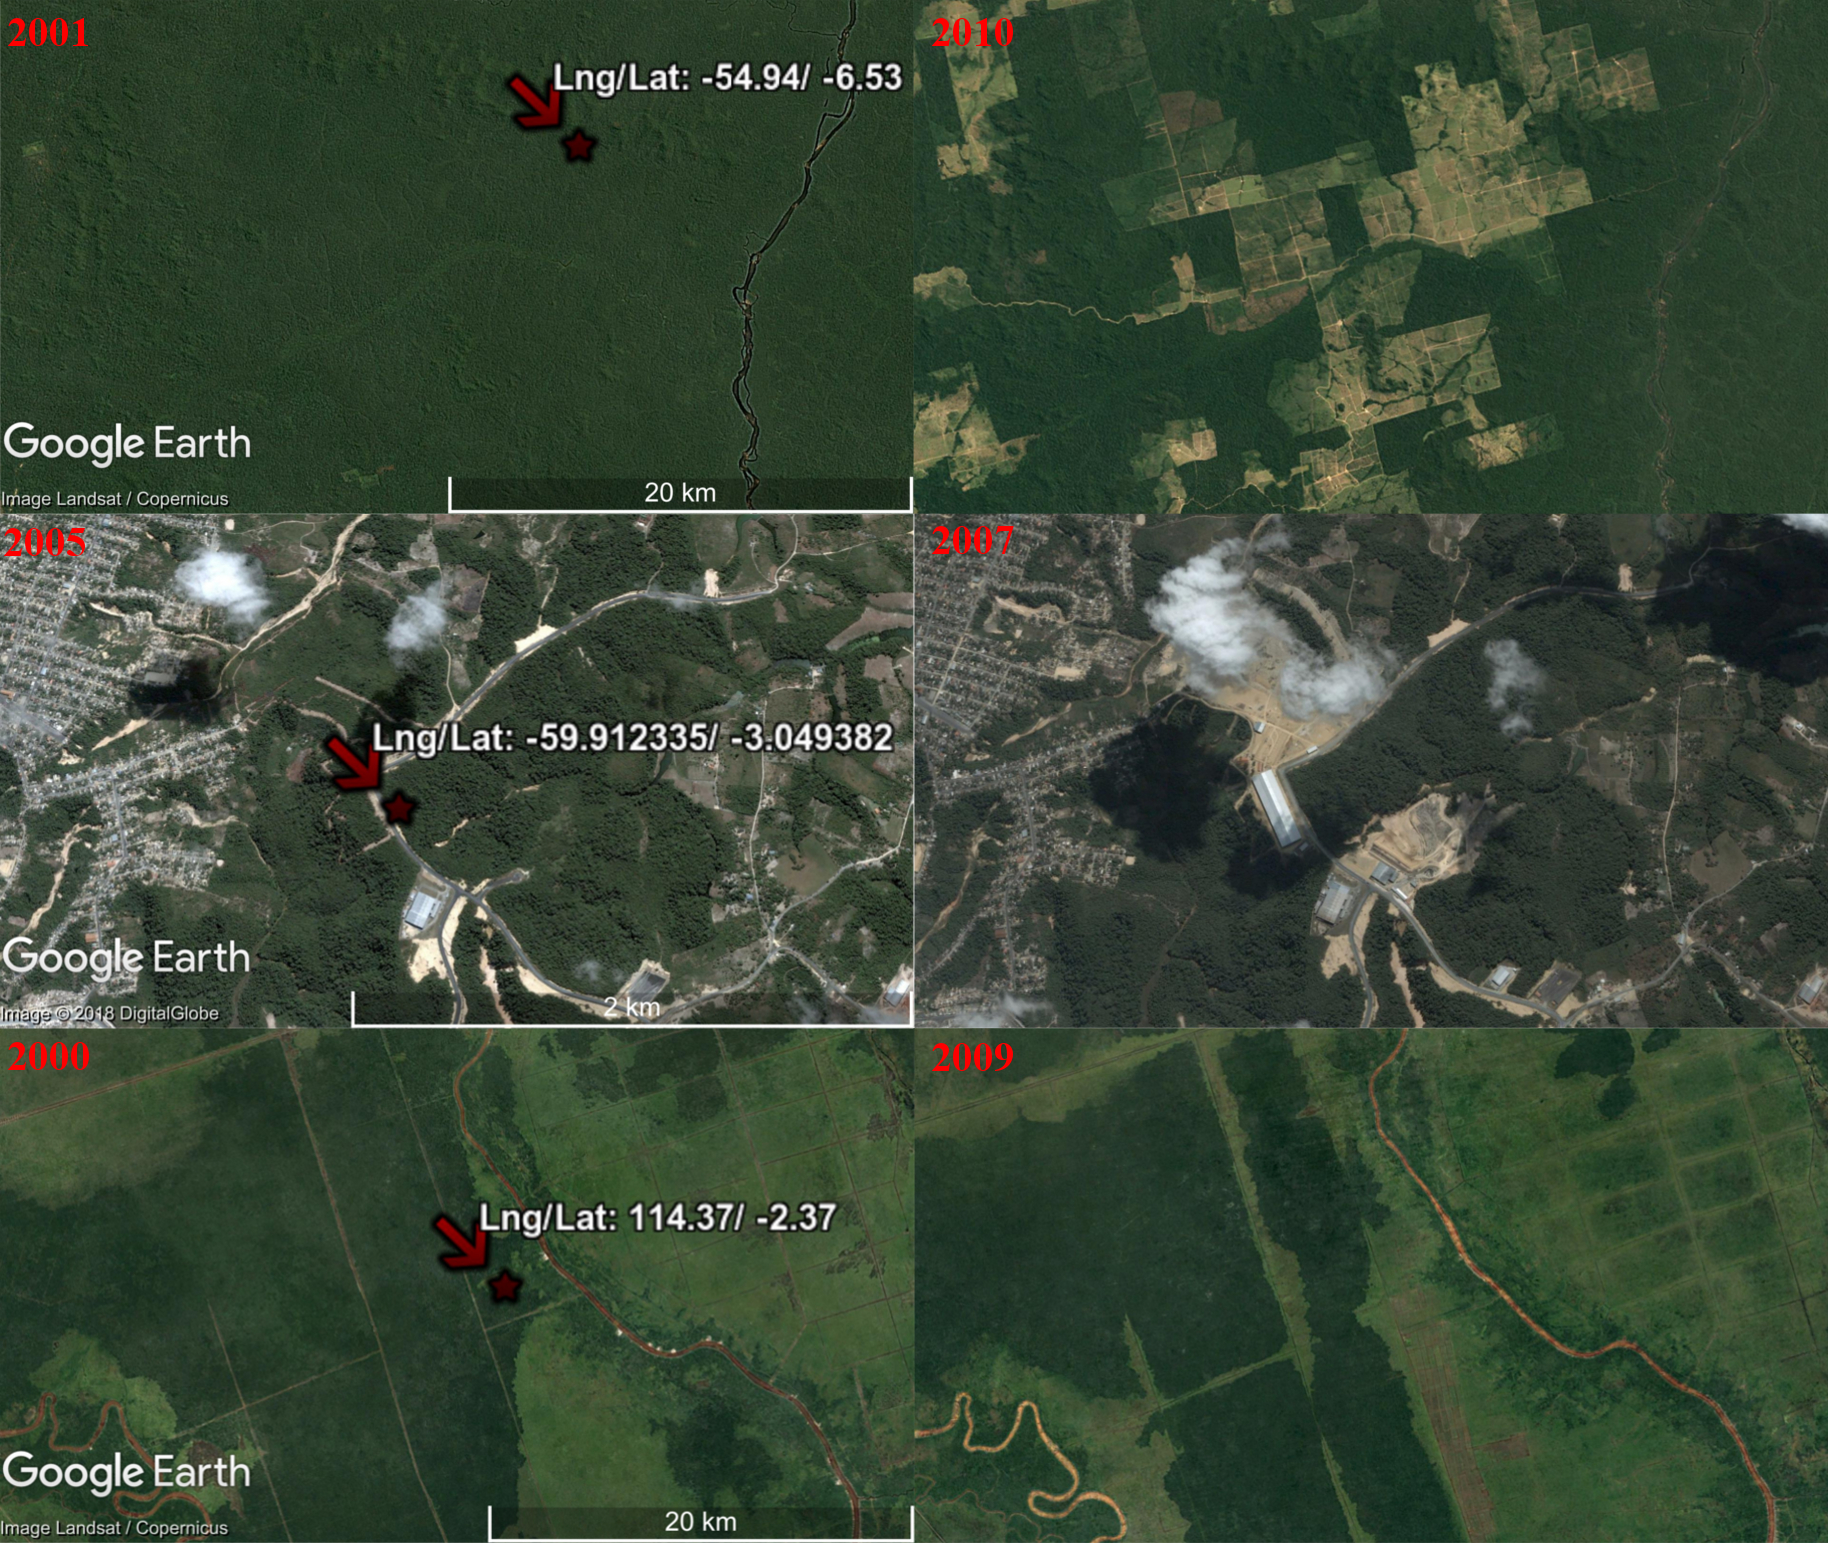
\includegraphics[scale=0.6]{img/deforestation_examples}
		\caption[Examples of proximate deforestation drivers]{\textbf{Examples of proximate deforestation drivers:} From top to bottom and left to right, pasture expansion in Brazilian rain forest, urban expansion in Brazil, and tree crop expansion in Indonesia.}
		\label{fig:deforestationexamples}
	\end{figure}

	\note{Emissions:} Deforestation not only changes land cover and drives the loss of biodiversity it also releases emissions. Some numbers. Mention the sources of emissions. No the gaps that agb estimates are common but soil organic carbon emissions are not estimated till no.

	Tropical forest ecosystems have a crucial impact on the well-being and subsistence of current and future generation out of humanity through the provision of regulatory, supporting, provisioning, and cultural services \citep{Costanza1997}. On the fact that deforestation and \ac{LC} changes lead to major changes in ecosystem services by altering the shape of forest biomes it is crucial to evaluate these impacts not only in terms of \ac{GHG} emissions but also for key ecosystem services as water, regulation, biodiversity etc. For the quantification of these ecosystem services a economic process is applied to assess the monetary value of each service per ecosystem. These \acp{ESV} can be a strong tool to determine the impact of certain management practices on ecosystem structures. Till now several studies prepared estimates of the \ac{ESV} loss by tropical deforestation by applying the global coefficients of \citeauthor{Costanza2014} \citep{Song2018,Costanza2014}. Further, several studies tried to estimate the \ac{ESV} changes by \ac{LULC} change dynamics on global and regional scale \citep{Costanza1997,Sannigrahi2018,Wang2006,Kreuter2001,Zhao2004}. Additionally, \citet{Groot2012} prepared a study on global \ac{ESV} dynamics by introducing alternative coefficients. To best of our knowledge no studies tried to determine the impact of \acp{PDD} on tropical forest cover in regards of \ac{ESV} change dynamics. \ac{ESV} change dynamics are defined by us as the \ac{ESV} loss by tropical deforestation, the \ac{ESV} gain by newly introduced \ac{LC} on former forested areas, and the \ac{ESV} net balance between both dynamics.

	\note{Research questions:}
	 Our goal is to develop an approach to determine spatially explicit the \acp{PDD} of tropical tree cover loss at a high spatial resolution. Our approach should meet the following criteria: high spatial resolution to consider for example small-holder deforestation; a easy accessible approach that can be reproduced without constraints; can be repeated by certain time steps in future. To achieve these goal we will combine the information from the most recent state of the art \ac{LC} datasets \ac{GFC} and \ac{GL30}.

	 Our goal is to evaluate theses dynamics by applying the most common in literature used \ac{ESV} datasets of \citeauthor{Costanza2014} and \citeauthor{Groot2012} at a global and continental scale between 2000 and 2010. Additionally we want to include the \ac{ESV} for tropical forest by the recent of study \citet{Siikamaki2015} to discuss differences between the three datasets. To compute the beforehand mentioned \ac{ESV} dynamics we will derive \ac{LC} change areas from our analysis on \acp{PDD} in the tropical zone.